\documentclass[11pt,a4paper]{article}
\usepackage[T1]{fontenc}
\usepackage{lmodern}
\usepackage[margin=2.2cm]{geometry}
\usepackage{graphicx,booktabs,microtype,xcolor,amsmath}
\usepackage[hidelinks]{hyperref}
\usepackage{enumitem}
\setlength{\parskip}{6pt}\setlength{\parindent}{0pt}
\newcommand{\code}[1]{\texttt{#1}}
% grey notes for the parts we have not written yet (remove at the end)
\newcommand{\todo}[1]{\textcolor{gray}{[TODO: #1]}}

\title{PDS 2026 -- Homework 1\\[2pt]
\large The t-SNE gradient on large graphs, in parallel}
\author{Code and raw data:
\url{https://github.com/mrsilentea07/graph-t-sne}}
\date{}

\begin{document}
\maketitle

% ------------------------------------------------------------
\section{The problem}

t-SNE draws a graph in the plane. Every node becomes a point, and nodes
that are connected should end up close to each other.

To get there, t-SNE moves the points a little at a time. The direction of
each move is the \emph{gradient}, and computing it is the task of this
homework. On every point act two forces:
\begin{itemize}
  \item an \textbf{attraction} towards its neighbours in the graph, and
  \item a \textbf{repulsion} away from all the other points.
\end{itemize}

The attraction only follows the edges, so it is cheap. The repulsion
involves every pair of points: for half a million nodes that is about
$3\cdot10^{11}$ pairs, which is far too many.

Before the forces, the edge weights are turned into a matrix $P$, which
says how strongly two neighbours attract each other.

We compute $P$ and the gradient once, at a given starting layout, for the
three graphs below. We wrote four versions: a sequential one, and parallel
ones in Pthreads, OpenMP and OpenCilk.

\begin{center}
\begin{tabular}{lrr}
\toprule
graph & nodes & stored edges \\
\midrule
\code{k49\_norm\_10NN} & 38{,}547  & 618{,}158 \\
\code{com-Amazon}      & 334{,}863 & 1{,}851{,}744 \\
\code{coPapersDBLP}    & 540{,}486 & 30{,}491{,}458 \\
\bottomrule
\end{tabular}
\end{center}

% ------------------------------------------------------------
\section{Our approach}

The work is done in four steps.

\begin{enumerate}
  \item \textbf{Compute $P$.} Each node (row) is handled on its own, so
    the rows are split among the threads.

  \item \textbf{Attraction.} For each node we add up the pull of its
    neighbours, again one row at a time. Some nodes have 1 neighbour and
    some have 3{,}299, so the rows are handed out to the threads as they
    become free, not in fixed blocks.

  \item \textbf{Repulsion (Barnes--Hut).} We put the points in a
    quadtree. Seen from far away, a group of points acts like a single
    point at its centre, so we do not visit every pair. This brings the
    cost down from about $n^2$ to about $n \log n$.
    The tree is built level by level, and then every point walks the
    tree on its own, in parallel.

  \item \textbf{Gradient.} We combine the two forces:
    gradient $= 4\,(\text{attraction} - \text{repulsion})$.
\end{enumerate}

All the computations are written once, in \code{src/tsne.h}. Each
parallel version only decides how the loops are divided among the
threads.

% ------------------------------------------------------------
\section{Setup}

\begin{itemize}
  \item \textbf{Machine:} laptop with an AMD Ryzen 7 6800HS, 8 cores /
    16 hardware threads, 16\,GB RAM, Ubuntu 24.04.
  \item \textbf{Compilers:} \code{gcc 13.3} for the sequential, OpenMP
    and Pthreads versions; OpenCilk 3.0 (\code{clang 19}) for OpenCilk.
    Flags: \code{-O3 -march=native}.
  \item \textbf{Method:} every phase is timed on its own. Each run is
    repeated 7 times and we keep the median. Settings: perplexity
    $u=10$, Barnes--Hut $\theta=0.5$, at most 16 points per tree leaf.
\end{itemize}

% ------------------------------------------------------------
\section{Correctness}

We compare our results with the reference files given with the homework.
The error is the largest difference divided by the largest value.

\begin{center}
\begin{tabular}{lccc}
\toprule
graph & $P$ and attraction & repulsion & gradient \\
\midrule
\code{k49\_norm\_10NN} & $1\cdot10^{-4}$  & $9\cdot10^{-3}$ & $8\cdot10^{-3}$ \\
\code{com-Amazon}      & $\approx 10^{-15}$ & $8\cdot10^{-3}$ & $3\cdot10^{-3}$ \\
\code{coPapersDBLP}    & $\approx 10^{-15}$ & $6\cdot10^{-3}$ & $2\cdot10^{-3}$ \\
\bottomrule
\end{tabular}
\end{center}

\begin{itemize}
  \item $P$ and the attraction match: up to the bisection tolerance on
    the weighted graph, and to round-off on the other two.
  \item The repulsion differs by less than 1\%. This is expected: we use
    Barnes--Hut with $\theta=0.5$, while the reference used the more
    accurate $\theta=0.1$.
  \item All four versions give the same numbers, with 1, 8 and 16
    threads (differences below $10^{-13}$, only from the order of the
    additions). ThreadSanitizer finds no data race.
\end{itemize}

% ------------------------------------------------------------
\section{Results}

\begin{figure}[h]
\centering
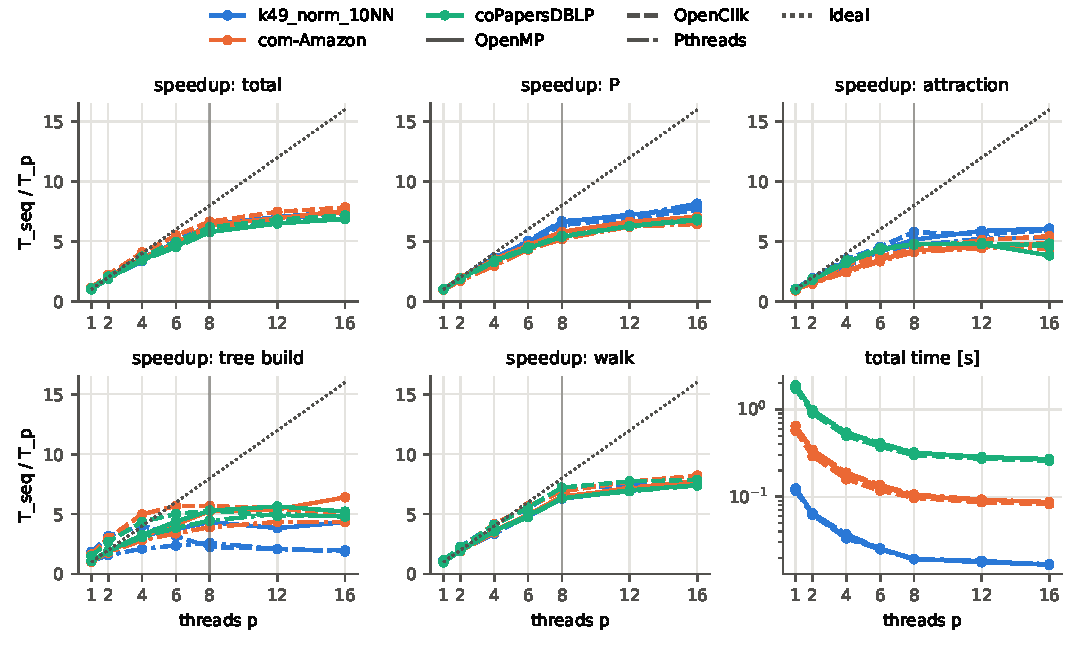
\includegraphics[width=\linewidth]{figs/scaling.pdf}
\caption{Speed-up of each phase over the sequential code, against the
number of threads. The vertical line marks the 8 physical cores.}
\label{fig:scaling}
\end{figure}

\begin{center}
\small
\begin{tabular}{lrrrr rrrr}
\toprule
 & \multicolumn{4}{c}{\code{com-Amazon}} & \multicolumn{4}{c}{\code{coPapersDBLP}} \\
\cmidrule(lr){2-5}\cmidrule(l){6-9}
time [ms], 16 threads & seq & omp & cilk & pthr & seq & omp & cilk & pthr \\
\midrule
$P$         & 54  & 7.6 & 7.8 & 8.4 & 846  & 125 & 123 & 124 \\
attraction  & 5.7 & 1.2 & 1.0 & 1.3 & 51   & 13  & 11  & 11  \\
tree build  & 12  & 1.9 & 2.5 & 2.8 & 24   & 4.5 & 4.9 & 4.9 \\
centers of mass & 0.7 & 0.2 & 0.2 & 0.4 & 1.6 & 0.4 & 0.4 & 0.5 \\
walk        & 570 & 73  & 69  & 74  & 927  & 125 & 118 & 126 \\
\midrule
total       & 644 & 85  & 82  & 87  & 1851 & 270 & 258 & 269 \\
\bottomrule
\end{tabular}
\end{center}

All three parallel versions run about \textbf{7 times faster} than the
sequential one, and they are within a few percent of each other.
What limits each phase:

\begin{itemize}
  \item \textbf{Walk} (the largest phase): scales best. Every point
    walks the tree on its own and the tree fits in the cache.
  \item \textbf{$P$:} scales well, but only if the rows are handed out
    dynamically. On \code{coPapersDBLP} a few rows are 3{,}000 times
    longer than others; with fixed blocks $P$ is 1.7 times slower.
  \item \textbf{Attraction:} stops at about 5 times. It mostly reads
    memory, and at 4--8 threads it already uses nearly all the memory
    bandwidth of the laptop.
  \item \textbf{Tree build and centers of mass:} the top levels of the tree have only 1, 4,
    16, \dots cells, so there is little to share. It is under 2\% of the
    total time, so it does not matter much.
  \item \textbf{More than 8 threads} give only 15--20\% more: the extra
    threads share the same 8 cores.
\end{itemize}

\textbf{Across the graphs}, the walk grows with the number of nodes and
$P$ with the number of edges. \code{coPapersDBLP} has many edges per node,
so there $P$ costs as much as the walk.

\textbf{Barnes--Hut vs.\ direct.} On \code{k49\_norm\_10NN} the direct
sum over all pairs takes 1.78\,s (sequential); Barnes--Hut takes
0.05\,s, about \textbf{40 times faster}. The direct sum only wins below
about 400 points (1{,}500 with 16 threads).

% ------------------------------------------------------------
\section{Predict, then measure}

Using only the two smaller graphs, we predicted each phase on
\code{coPapersDBLP}: $P$ and attraction grow with the edges, the tree with
the nodes, the walk with $n\log n$.

\begin{center}
\begin{tabular}{lrrrr}
\toprule
 & \multicolumn{2}{c}{sequential [ms]} & \multicolumn{2}{c}{OpenMP, 8 threads [ms]} \\
 & predicted & measured & predicted & measured \\
\midrule
$P$        & 889  & 846  & 153 & 157 \\
attraction & 76   & 51   & 17  & 11  \\
walk       & 955  & 927  & 147 & 147 \\
\midrule
total      & 1941 & 1851 & 321 & 320 \\
\bottomrule
\end{tabular}
\end{center}

The total was right within 5\%. The attraction was over-estimated by
50\%: part of its cost is per row, not per edge, and \code{coPapersDBLP}
has many more edges per row, so this part weighs less.

% ------------------------------------------------------------
\section{One bug}

The tree can have up to 21 levels, but the array that stores where each
level starts was one entry too short. The small graph never got that deep,
but \code{com-Amazon} did, because many of its points fall on almost the
same spot. The results were still correct, so the comparison with the
reference could not show it. We found it by checking the loop limits, and
confirmed it with AddressSanitizer (\code{-fsanitize=address}). The fix
was one more entry in the array.

% ------------------------------------------------------------
\section{Sources and AI assistance}

Van der Maaten, \emph{Accelerating t-SNE using tree-based algorithms},
JMLR 2014; Barnes and Hut, Nature 1986; the OpenMP and OpenCilk
documentation.
An AI assistant (Claude) wrote most of the code, in particular the
Pthreads version, from a design that we worked out together; we checked
every result against the reference and the measurements. It made
mistakes such as the bug above, which we had to catch.

\end{document}
